\section{Introduction}
\label{sec:introduction}
%%% General intro
The exponential improvement in computing performance and the availability of large amounts of data are boosting the use of \gls{ai} applications in our daily lives. Among the various algorithms developed over the years, neural networks have demonstrated remarkable performance in a variety of image, video, audio, and text analytics tasks~\cite{schmidhuber2015deep,Taigman_2014_CVPR}. Historically, \glspl{ann} can be classified into three different generations \cite{Design_Exploration_SbS_Trans20}: the first one is represented by the classical McCulloch and Pitts neuron model using discrete binary values as outputs; the second one is represented by more complex architectures as \gls{mlp} and \gls{cnn} using continuous activation functions; while the third generation is represented by \gls{snn} using spikes as means for information exchange between groups of neurons. Although the \gls{ai} research is currently dominated by \glspl{dnn} from the second generation, the \glspl{snn} belonging to the third generation are receiving considerable attention \cite{Spinnaker_Trans13,ernst2007efficient,Design_Exploration_SbS_Trans20, SNN_Survey_Trans19}.

\glspl{snn} offer advantageous robustness and the potential to achieve a power efficiency closer to that of the human brain.
%%%
\glspl{snn} operate reliably using stochastic elements that are inherently non-reliable mechanisms \cite{mcdonnell2011benefits}.
This provides superior resistance against adversary attacks
\cite{ernst2007efficient, Dapello2020.06.16.154542}. Beside
robustness, \glspl{snn} have further advantages like the possibility of a more efficient asynchronous parallelization and higher
energy efficiency than \glspl{dnn}. For
example, Loihi \cite{davies2018loihi}, a \gls{snn} developed by Intel, can
solve LASSO optimization problems with an over three orders of
magnitude better energy-delay product than conventional
approaches. These advantages are motivating large research programs by
major companies (e.g., Intel \cite{davies2018loihi} and IBM
\cite{TrueNorth_Trans15}) as well as pan-european projects in the
domain of spiking networks \cite{Spinnaker_Trans13}.


\glspl{snn} emulate the real behavior of neurons in different levels of detail. The more detailed the biological part is emulated, the greater the computational complexity \cite{izhikevich2004model,amunts2019human}. For example, \gls{lif} is a widely used model; however, this model is relatively complex for emulation in embedded applications.
	
	Alternatively, the \gls{sbs} neural network is a remarkable model for its reduced complexity, which is on the less realistic side of the \gls{snn} scale of biological realism~\cite{rotermund2019Backpropagation,ernst2007efficient}. Consequently, the hardware complexity of \gls{sbs} network implementations is greatly reduced
	\cite{nevarez2020accelerator,rotermund2018massively}. In spite of this, \gls{sbs} still uses stochastic spikes as a means of transmitting information between populations of neurons and thus retains the advantageous robustness of \glspl{snn}.


%%% SbS intro
%SbS neural networks \cite{rotermund2019back,ernst2007efficient} are inspired by the %natural information processing of the mammalian brain.
The conceptual model in \gls{sbs} (see Chapter~\ref{sec:sbs} for a review) differs fundamentally from conventional \glspl{ann} since (a) the building blocks of the network are \glspl{ip_sbs} which are an optimized generative representation with non-negative values, (b) time progresses from one spike to the next, preserving the property of stochastically firing neurons, and (c) a network has only a small number of parameters, which is an advantageous noise-robust stochastic version of \gls{nnmf}. The \gls{sbs} network is placed between non-spiking \glspl{nn} and stochastically spiking \glspl{nn}, which offers advantages from both structures \cite{rotermund2019Backpropagation}. On one hand, the \gls{sbs} model incorporates the inherent robustness of \glspl{snn}, which provide the possibility of more efficient asynchronous parallelization and superior resilience against disturbances based on the synaptic stochasticity; on the other hand, the \gls{sbs} model incorporates the regular flow of information from \glspl{cnn}, which are expressed on explicit vector operations.  


%%%%%%% Problem statement
As computational demanding algorithms, \glspl{cnn} and \glspl{snn} in particular, must be addressed by specialized hardware architectures. A significant research effort has been performed in \gls{snn} accelerators, see e.g.~\cite{roy2019towards,bouvier2019spiking, young2019review,TrueNorth_Trans15,Spinnaker_Trans13,davies2018loihi}.
  However, hardware accelerators that focus on \gls{sbs} have only been partially investigated so far~\cite{nevarez2020accelerator,rotermund2018massively}.
  Enhanced \gls{sbs} accelerators will have a double impact. From the application point of view, they will contribute to the deployment of robust neural networks in small embedded systems~\cite{nevarez2020accelerator}; from the scientific point of view, they will facilitate fundamental research for neuroscience~\cite{ernst2007efficient,rotermund2019recurrentsbs, dayan2001theoretical}.

A central point that can be optimized in current \gls{sbs} accelerators
is the use of approximation techniques.
Most \gls{sbs} models use \gls{fp}  numerical representation, which imposes high complexity of the required circuits for the \gls{fp} operations. Model quantization has the potential to improve computational performance; however, this solution is often accompanied by quantization-aware training methods that, in some cases, are problematic or even inaccessible, particularly in deep \gls{snn} algorithms~\cite{zhang2018survey}. 
As an alternative, based on the relaxed need for fully precise or deterministic computation of neural networks, approximate computing techniques allow substantial enhancement in processing efficiency with moderated accuracy degradation. Some research papers have shown the feasibility of applying approximate computing to the inference stage of neural networks~\cite{lotrivc2012applicability, sarwar2016multiplier, mrazek2016design, du2014leveraging}. Such techniques usually demonstrated small inference accuracy degradation, but significant enhancement in computational performance, chip-area, and energy consumption. Hence, by taking advantage of the intrinsic error-tolerance of neural networks, approximate computing is positioned as a promising approach for inference on resource-limited devices.

\begin{figure*}[b!]
	\centering
	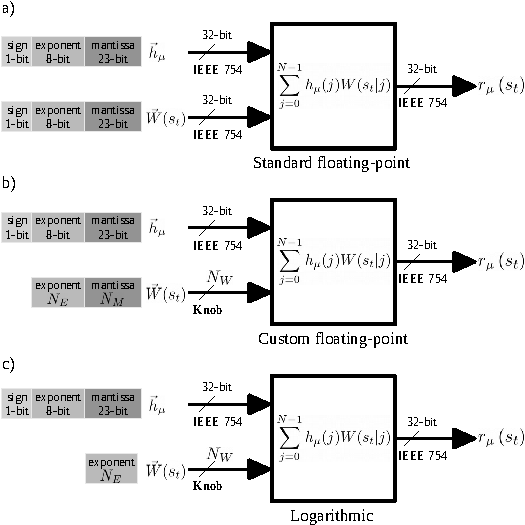
\includegraphics[width=0.5\columnwidth]{./chapters/sbs_accelerator/figures/dot-product_unit.pdf}
	\caption{Dot-product hardware module with (a) standard floating-point (IEEE 754) arithmetic, (b) hybrid custom floating-point approximation, and (c) hybrid logarithmic approximation.}
	\label{fig:dot_product_unit}
\end{figure*}

%%%%%%% Contributions
In this chapter, we accelerate \gls{sbs} neural networks with a dot-product hardware design based on approximate computing with hybrid custom \gls{fp}  and logarithmic number representation. This hardware unit has a quality configurable scheme based on the bit truncation of the synaptic-weight vector. \Fig{fig:dot_product_unit} illustrates the dot-product hardware module with standard \gls{fp} (IEEE 754) arithmetic, and our approach with hybrid custom \gls{fp}  as well as logarithmic approximation. As a design parameter, the mantissa bit-width of the weight vector provides a tunable knob to trade-off between efficiency and \gls{qor}~\cite{park2009dynamic, han2013approximate}. Since the lower-order bits have smaller significance than the higher-order bits, truncating them may have only a minor impact on \gls{qor}~\cite{gupta2011impact, mittal2016survey}. Further on, we can remove completely the mantissa bits in order to use only the exponent of a \gls{fp}  representation. Therefore, the most efficient setup and yet the worst-case quality configuration becomes a logarithmic representation, which consequently leads to significant architectural-level optimizations using only adders and shifters for dot-product approximation in hardware. Moreover, since approximations and noise have qualitatively the same effect~\cite{venkataramani2015approximate}, we apply noise tolerance plots as an intuitive visual measure to provide insights into the quality degradation of \gls{sbs} networks under approximate processing effects.

The main contributions in this work are as follows:

\begin{itemize}
	\item We develop a hardware component for dot-product approximation. To perform the sum of pairwise products of two vectors, this hardware module has the following three design features: (1) the pairwise product is approximated by adding integer exponents and multiplying truncated mantissas, and the sum of products is done by accumulating denormalized integer products with barrel shifters, which increases computational throughput; (2) the synaptic weight vector uses either reduced custom \gls{fp} or logarithmic representation, which reduces memory footprint; and (3) the neuron vector uses either standard or custom \gls{fp} representation, which preserves \gls{qor} and overall inference accuracy.
	\item We address a hardware design exploration with the proposed dot-product approximation using synaptic weight vectors with custom \gls{fp} and logarithmic representation as shown in \Fig{fig:dot_product_unit}. We evaluate inference run-time, accuracy degradation, resource utilization and power dissipation. Experimental results demonstrate $20.5\times$ run-time enhancement versus embedded CPU (ARM Cortex-A9 at \unit[666]{MHz}), and less than $0.5\%$ of accuracy degradation without retraining on a handwritten digit recognition task (MNIST). This machine learning task simply provides a proof of concept to demonstrate the feasibility of our approximation technique for \gls{sbs} neural network accelerators.
	\item We propose a noise tolerance plot as quality monitor, which serves as an intuitive visual model to provide insights into the accuracy degradation of \gls{sbs} networks under approximate processing effects.
	\item Our proposed design for dot-product approximation is adaptable as a building block for other error resilient applications (e.g., image/video processing).
\end{itemize}

To promote the research on \gls{sbs} networks, our design exploration framework is made available to the public as an open-source project at https://github.com/YaribNevarez/sbs-framework.git

